%!TEX root = ../dissertation.tex
\begin{savequote}[75mm]
Before anything else, preparation is the key to success.
\qauthor{Alexander Graham Bell}
\end{savequote}

\chapter{Preparation}
\section{A11Y Guide}
In preperation for the main deliverable a deeper level of knowledge in the
accessibility space was required. To gain this knowledge and inline with my
'Share Everything' approach it was decided that an 'Accessibility
training guide' would be produced here on referred to as 'A11Y guide'. The idea
being that in producing a guide for others, oneself would have to be
knowledgable enough to produce good content.

\subsection{Planning}
% TODO - Reference curve: http://www.wranx.com/ebbinghaus-and-the-forgetting-curve/

As researched by Ebbinghaus in 1885 the forgetting curve demonstrates the
amount of knowledge remembered after a period of time. see Fig.~\ref{fig:ebbinghaus}
Repeating or revising the learning unsuprisingly results in the knowledge
stored in memory for longer.

\begin{figure}
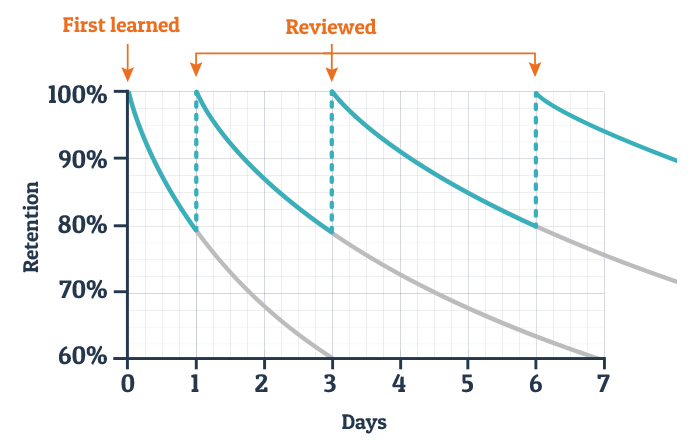
\includegraphics[width=\textwidth]{figures/ebbinghaus}
\caption[Short figure name.]{Ebbinghaus' famous forgetting curve
\label{fig:ebbinghaus}}
\end{figure}

With this in mind I plan to iteratively build the A11Y Guide so
that the knowledge will be reinforced. The steps for its production will be
as follows:
\begin{enumerate}
  \item Search for useful resources online (This will be first time learning)
  \item Score the identified resources with the assistive tools for a first hand
  experience along with other criteria (This second time repeating)
  \item Collate the resources under the correct header in a github project
  \item Setup continuous deployment scripts to ensure deploy on commit
  \item For each header create and document best practices (This third time
  repeating)
  \item Build a basic documentation website
  \item For each header create coded examples (This fourth time repeating)
\end{enumerate}

As explicitly stated there will be four loops of observing, reviewing and
applying the knowledge learned which should result in a peak knowledge level
when producing the tool.

\subsection{Building A11Y Guide Requirements}
In parallel to the above, for the guidance to have a greater impact it
needs to be current, relevant and available. This will require some additional
work to research the current state of web frameworks and also the
requirements of Capgemini's teams. To do this I propose issuing a
questionnaire to my colleagues and using google trends to gain an
understanding of the direction
of front end web development.

\subsubsection{Understanding industry movement}
% TODO
% - Reference State of JS

\subsubsection{Questionnaire}
% TODO
% - Reference Professional competency scale https://hr.od.nih.gov/workingatnih/competencies/proficiencyscale.htm
% - Reference Remote working Capgemini
% - Reference google forms

Capgemini employees are typically engaged on client sites across the country
resulting in the need for the questionnaire to be digital. To increase
the possible respondants and not affect current work it will need to be
completable in ~2-4 minutes. This will limit the number of questions and the
type of questions that can be used.

The aim of the questionnaire is to gain a wider understanding of the
frameworks, components and level of accessibility knowledge across a variety
of software engineers that work in different areas (Front End, Java, PHP,
etc). Due to the limited time for respondants to answer questions and the
aim of the information I believe Quantative data is best for this purpose.

Google Forms is to be used to implement the questionnaire due to its simple
setupand integration into Google Spreadsheets which will make analysis simpler.

\textbf{Question 1 - What JS frameworks is your current project
using?}

This question is required to gather evidence of what frameworks clients are
having Capgemini build their products in. The data produced from this
question will be used to understand the current climate.

This question will be multi-choice with the option of adding 'other' in which
case a textual box will be displayed. An answer will be required.

\textbf{Question 2 - What JS frameworks would you consider yourself
competent in?}

As the A11Y guide will hold coded examples there is a need to understand what
frameworks developers are competent in. If they consider themselves competent
they should be able to understand examples using it and apply them to their
current project work. The answers to this will likely determine what
framework is used when producing specific guidance.

Similarly to above this question will use the same list of frameworks.

\textbf{Question 3 - Which of the following Styling Frameworks do you
use/actively recommend ?}

Styling Frameworks add CSS and often developers copy and paste the examples
given on the Styling Frameworks website. If people are using certain
frameworks they may be inadvertently following some of the best practices. I
want to name and shame the good and the bad frameworks for accessibility so
new project set off on a good start.

Also multi-choice and required.

\textbf{Question 4 - What additional libraries are you using?}
This will be a 'textual' input field and in the description users will be
advised they can paste a 'package.json' file in (A common method of managing
dependencies in a javascript project). This will be an optional question to
promote people to complete the questionnaire.

\textbf{Question 5 - What form items does your project use?}
Coming back to relevancy for the A11Y guide, content will be produced for the
highest ranking form items first. This will ensure that if the guide is not
100\% complete it will still likely add a lot of value to Capgemini.

This question will be multi-choice and list a range of different methods of
user input

\textbf{Question 6 - What Web Components does your project use?}
Similar to above accept it is probably within the scope of this project that
only the highest ranking six will have guidance produced. This may be
completed however after the project.

\textbf{Question 7 - What level would you consider your web accessibility
level?}
This question aims to have the developer place themselves on the NIH
Proficiency Scale. It will have some additional guidance to help them
position themselves:
\begin{itemize}
\item None
\item Fundamental Awareness - Know what it is, but not how to implement it
\item Novice - Can implement with help from Google
\item Intermediate - Can implement with help and has experience testing with tools such as JAWS, Dragon
\item Advanced  - Can implement without help, understands \& explains how.
Knows best practice
\item Expert - The 'go to' person for web accessibility
\end{itemize}

This is probably the most important question. The answers to this will
determine the depth to which the guidance goes into, and also it's
recommended usage.

\subsubsection{A11Y Guide Requirements}
The following requirements will be used to determine the success and evaluate
the solution. They have come from the results of the questionnaire and inline
with the manifesto of the project:
\begin{itemize}
\item Contain output 'snippets' from the tools
\item Use React for coding examples
\item Use Material UI when styling or a specific framework is expected
\item
\end{itemize}

\subsection{Gathering Knowledge}
This section will describe the methods and results of gathering resources to
be used to support the A11Y Guide.

\subsubsection{Method}

\subsubsection{Scoring}
\subsubsection{Outputs}

\subsection{Building the A11Y Guide}
% TODO
% - Reference mockups
\subsubsection{Iteration 1 - Create content using markdown}

\subsubsection{Iteration 2 - UI Design \& Build site}
I wanted the UI to be simple and follow all the best practices it recommends.
As I had written some content it made it easier to experiment and understand
what was needed. The content was structured almost as a hierarchichal tree so
some sort of accordian type navigation would be useful. The audio snippets
would need to supplement the main content. The code snippets
would need to be compiled and embeddedable in the page.

I used moqups to produce a three different designs.

Design 1:

Design 2:

Design 3:

I chose design three...

\subsubsection{Iteration 3 - Continue content}
\subsubsection{Iteration 4 - Recognise/Implement custom pages}
\subsubsection{Iteration 5 - Continue content}
\subsubsection{Iteration 6 - Generify}

\subsection{Extending the impact}
\subsubsection{Colour Contrast Tool}
\subsubsection{Markdown/React Documentation Framework}

\section{A11Y Analysis Tool}
\subsection{Requirements}
\subsection{Diagrams}
\subsection{Design}

\section{Additional }
% TODO - discuss Travis CI for report writing
% TODO - discuss Branching model
% TODO - discuss any Standards


Principally, this chapter should describe the work that was undertaken before
code was written, hardware built, theories worked on, or research studies
executed. It should show how the project proposal was further refined and
clarified, so that the implementation/research execution stage could go
smoothly rather than by trial and error. This part of the report is attempting to
prove that you went through a planning process before embarking on the
deliverable so among others it might include discussion of:

1. For software projects, a requirements analysis, HCI designs, architectural
and use-case diagrams, etc.
2. Any programming languages learnt, any complicated theories or algorithms
that required understanding
3. For research-based projects, the research approach (experimental design,
where applicable), including methods and tools that were used/applied. If the
research method involves the development of prototypic software to test a
concept, briefly describe the design, structure, and creation of this software.
Research methods should be described such that a third party could replicate
the study/experiment to validate the results.

This section should be answering the question “How did I plan to achieve the
deliverable?”
